%!TEX root = ../Thesis.tex
\chapter{predictPotency}

blllaaah
\begin{figure}[ht]
\label{devel_fassif}
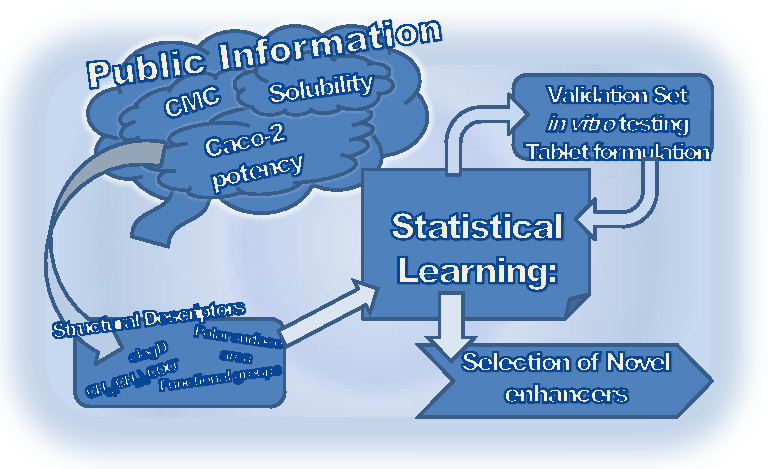
\includegraphics{graphics/workSummary_130mm.pdf}
\caption{Project idea. This figure was first designed for PhD-related presentations given by the author.}
\end{figure}


\begin{figure}[ht]
\label{devel_fassif}
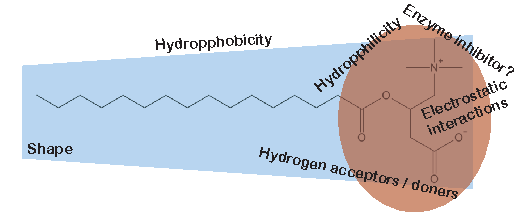
\includegraphics{graphics/typeOfSurfactant.pdf}
\caption{how does a surfactant like enhancer look like. This figure was first designed for PhD-related presentations given by the author.}
\end{figure}

\begin{figure}[ht]
\label{devel_fassif}
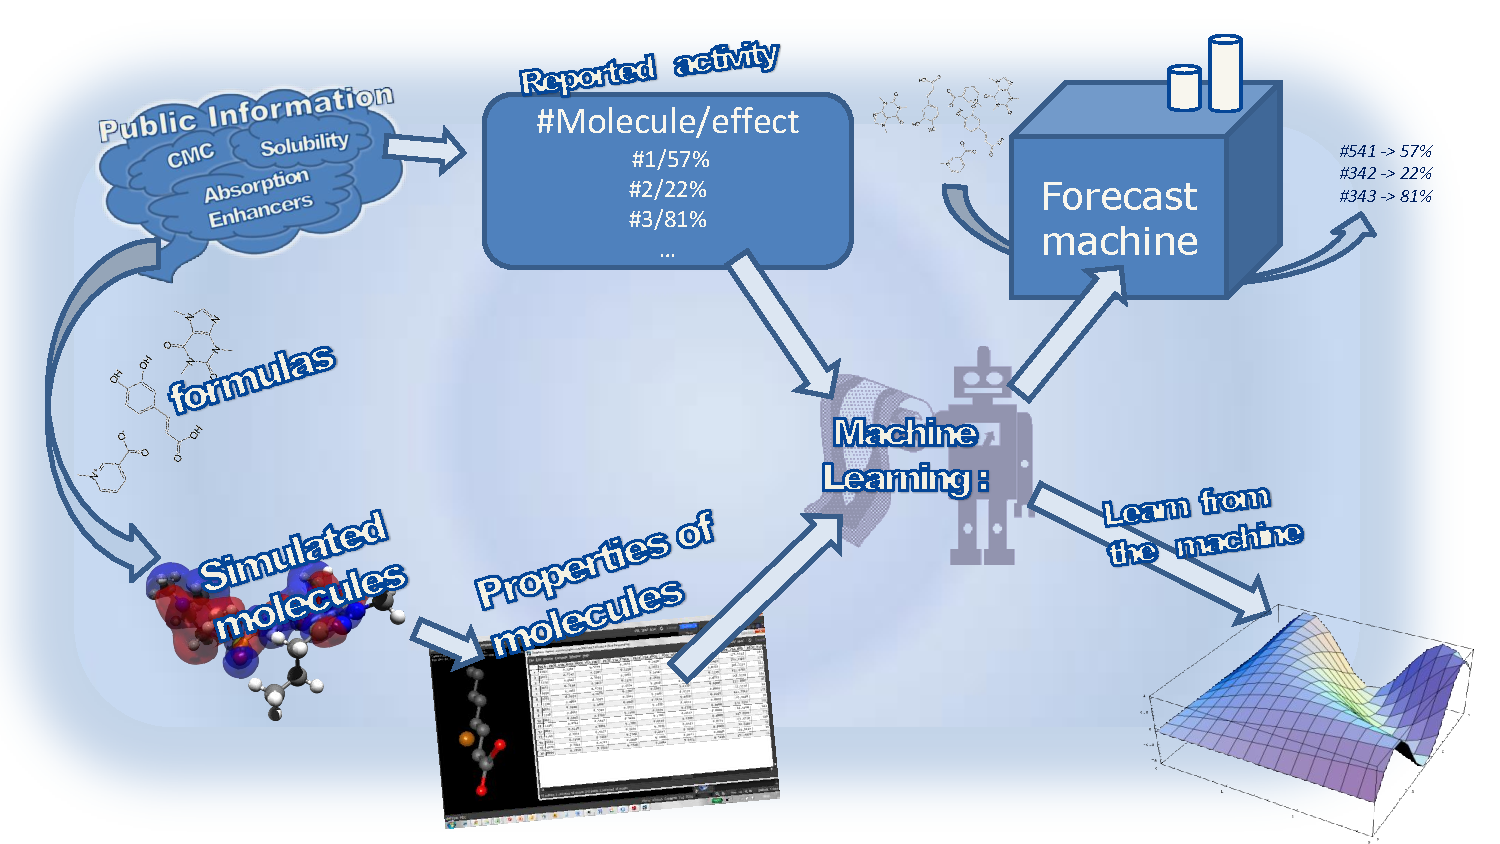
\includegraphics[width=\textwidth, height=\textheight, keepaspectratio]{graphics/predictPotencySummary.pdf}
\caption{Outline how to predictions are made. This figure was first designed for PhD-related presentations given by the author.}
\end{figure}

The decision tree ensemble random forest have a series of useful diagnostics which have been used in this thesis work.

\newpage

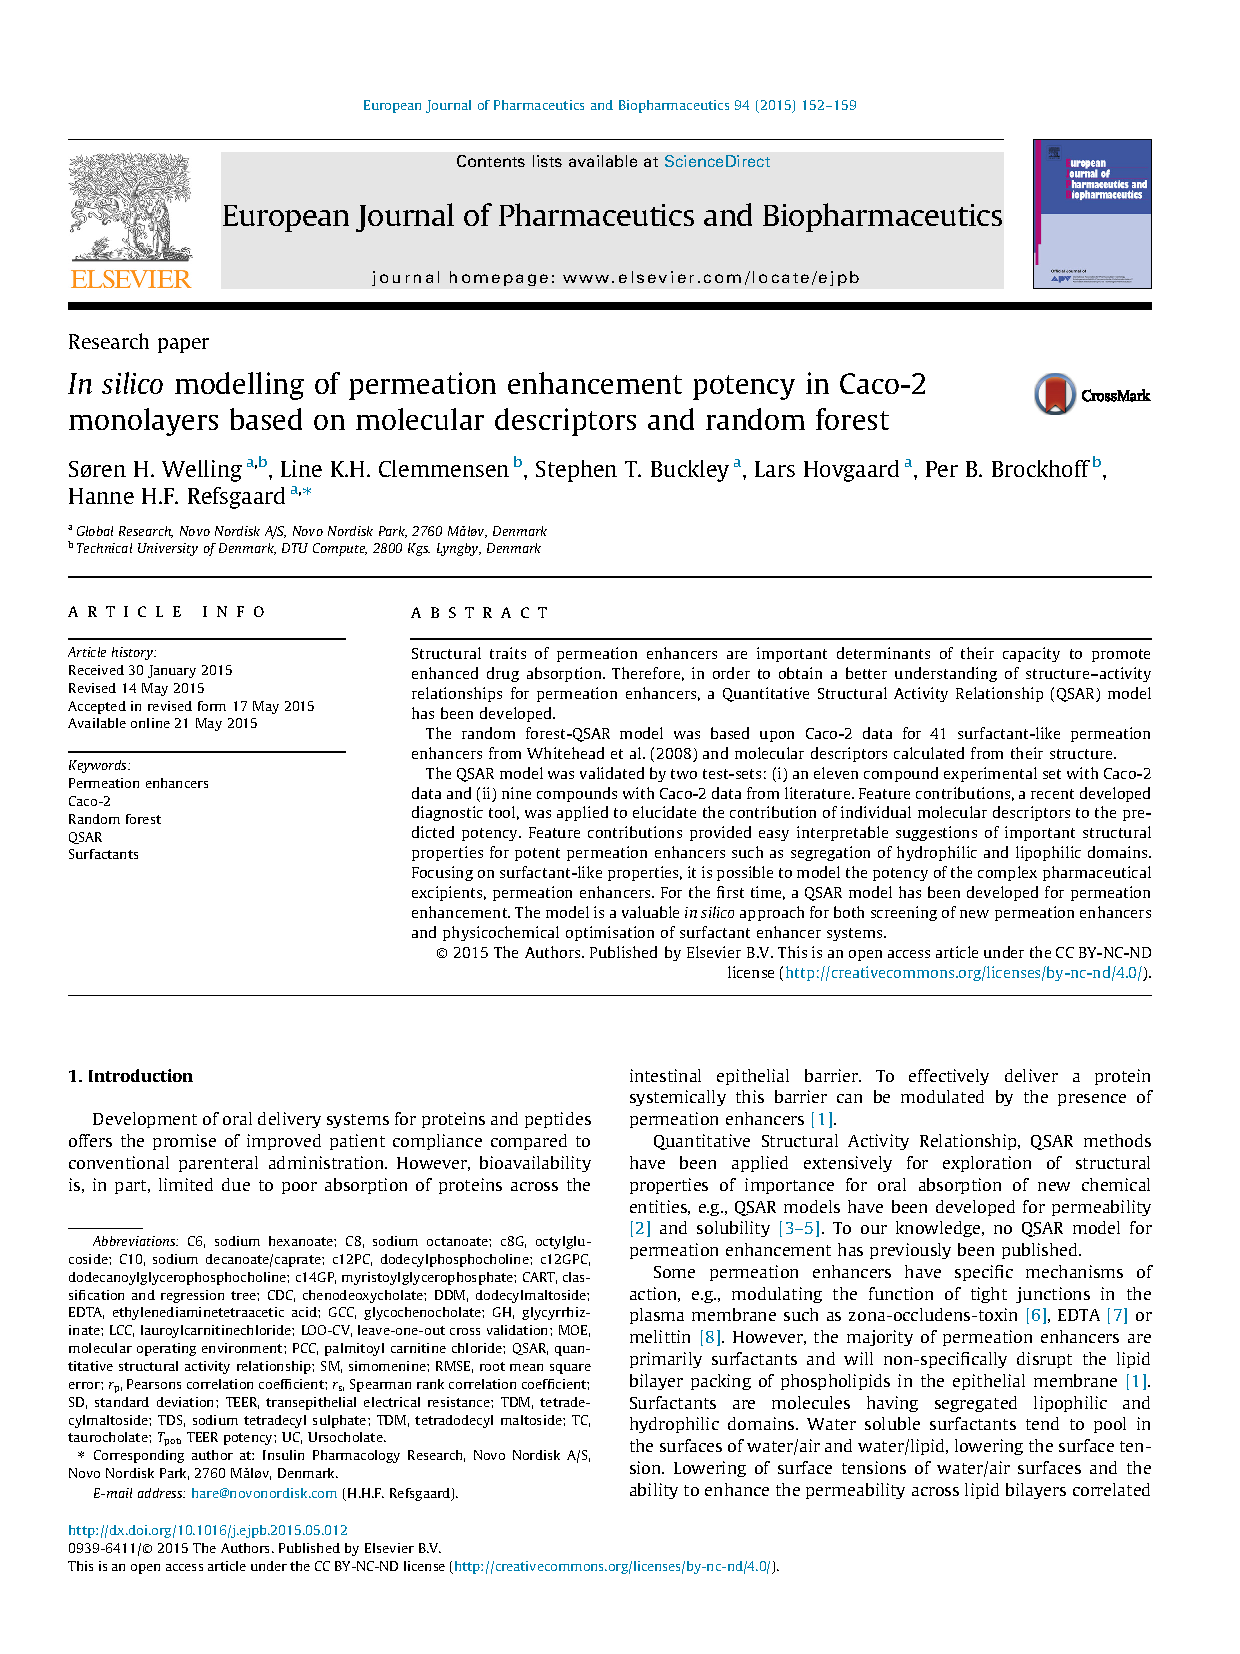
\includepdf[pages={1-},scale=0.90,pagecommand={\pagestyle{myruled}}]{chapters/predictPotencyArt.pdf}
